%\begin{itemize}
%\item so we had a focus group to actually elaborate the aprroach
%\item then we used explorative prototyping to elicit the initial version of the prototype and then refined that by means of case study, we could mention that we used ATC as an action-research source (this is what we are doing now internally in WP2 actually)
%\item ...
%\end{itemize}

The work we elaborated in this paper is stemming from the following research question:

\begin{center}
\emph{``How can we assist the continuous architecting of stream processing systems?"}
\end{center}

\comment{I would say if we connect it to the special need in DICE would makes more sense?}
The results contained in this paper in response to this research question were initially elaborated within a free-form focus group \cite{focusgroup} involving three experienced practitioners and researchers on big data streaming technologies, such as Storm. Following the focus group, through self-ethnography \cite{selfeth} and brainstorming we identified the series of essential consistency checks, algorithmic evaluations as well as anti-patterns that can now be applied through OSTIA while recovering an architectural representation for Storm topologies. We designed OSTIA\footnote{\url{https://github.com/maelstromdat/OSTIA}} to support the incremental and iterative refinement of streaming topologies based on the incremental discovery and correction of the above checks and patterns.

\begin{figure*}
\begin{center}
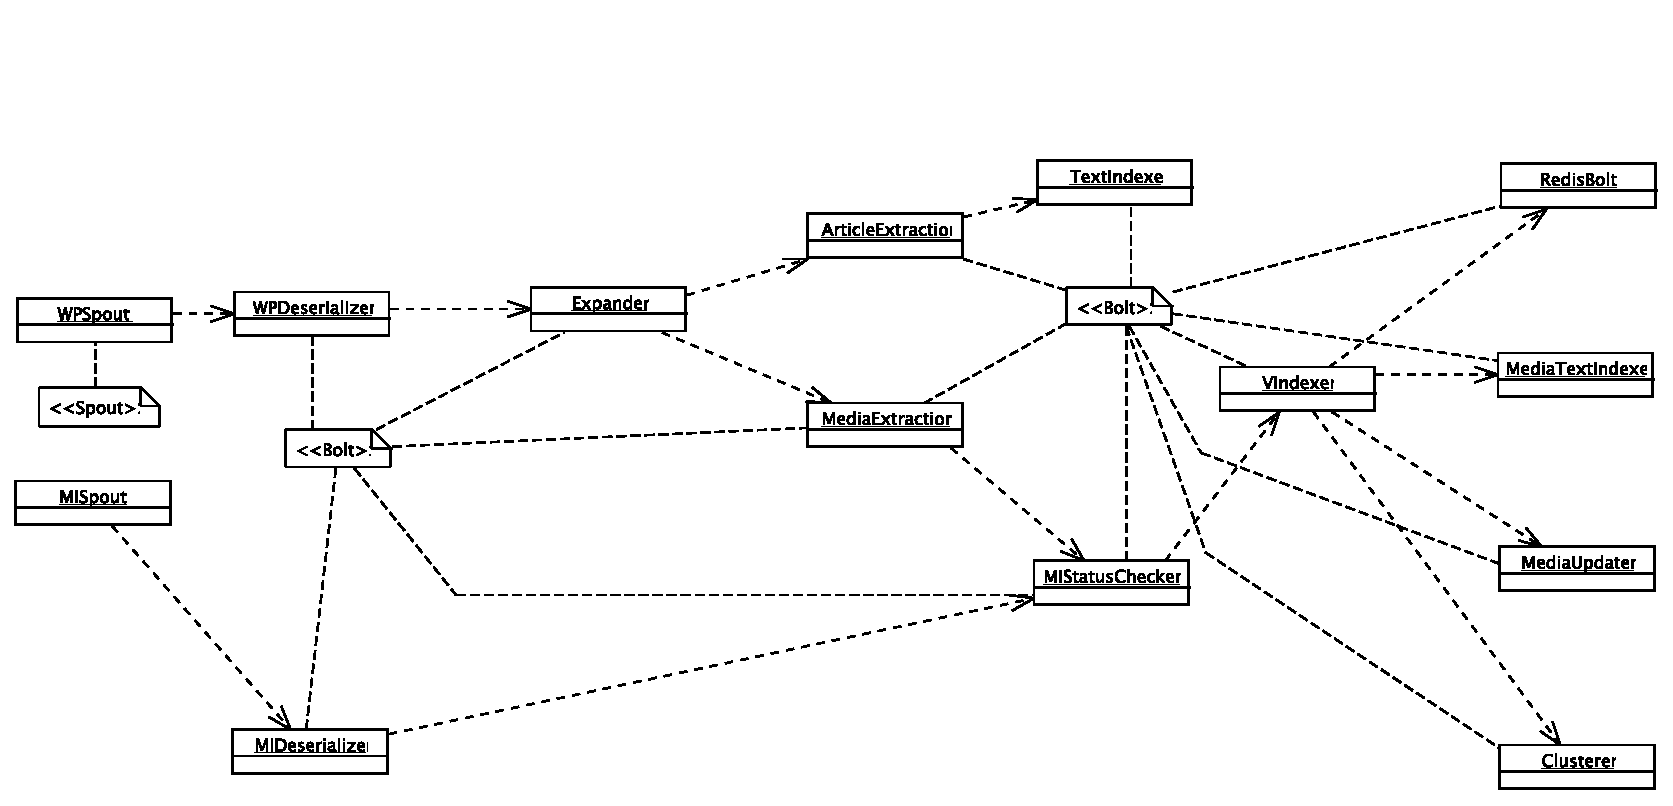
\includegraphics[width=12cm]{images/socialsensor}
\caption{A sample Storm topology in the SocialSensor App.}
\end{center}
\label{topo1}
\end{figure*}

In addition, we incrementally refined and evaluated OSTIA through scenario-analysis and case-study research \cite{casestudy} involving an industrial partner.

As previously stated, OSTIA was evaluated by means of an industrial case-study \comment{wasnt it three?} offered by one of the industrial partners in the DICE EU H2020 Project consortium\footnote{\url{http://www.dice-h2020.eu/}}. 
The partner in question uses open-source social-sensing software to elaborate a subscription-based big-data application that: (a) aggregates news assets from various sources (e.g., Twitter, Facebook, etc.) based on user-desired specifications (e.g., topic, sentiment, etc.); (b) presents and allows the manipulation of data. Said \comment{I'm not sure using ''said'' is formal?} application is based on the SocialSensor App\footnote{\url{https://github.com/socialsensor}} which features the combined action of three complex streaming topologies based on Apache Storm (see Fig. \ref{topo1} for a sample).

In particular, the topology in Fig. \ref{topo1} extracts data from sources and manipulates said data to divide and arrange contents based on type (e.g., article vs. media), later updating a series of databases (e.g., Redis) with these elaborations. The models that OSTIA elicited from this application were showcased to our industrial partner in a focus group aimed at establishing the value of insights produced as part of OSTIA-based analyses. Our qualitative assessment was based on questionnaires and open discussion.

To further validate OSTIA on open-source projects, we applied it on two open-source applications featuring Big-Data analytics and built on top of the Storm streaming technology, namely: (a) the DigitalPebble application, i.e., quoting from the homesite\footnote{\url{https://github.com/DigitalPebble/storm-crawler}}, ``A Text Classification API in Java originally developed by DigitalPebble Ltd. The API is independent from the ML implementations used and can be used as a front end to various ML algorithms"; (b) the StormCV application, i.e., quoting from the homesite\footnote{\url{https://github.com/sensorstorm/StormCV}} ``StormCV enables the use of Apache Storm for video processing by adding computer vision (CV) specific operations and data model; the platform enables the development of distributed video processing pipelines which can be deployed on Storm clusters".

%\begin{itemize}
%\item elaborate on the case-study partner
%\item elaborate on the case at hand for that partner
%\item elaborate on the origin of the application and how it uses social-sensor
%\item also, elaborate on the case by NETF which starts and stems from KILLRWEATHER
%\item should we elaborate on something else?
%\end{itemize}
%\textbf{TODO: @anyone, feel free to elaborate more!!}

Finally, we applied well-established verification approaches to integrate the value and benefits behind using OSTIA. We engineered OSTIA to support exporting of elicited topologies for their further analysis using the Zot\footnote{\url{https://github.com/fm-polimi/zot}} LTL model-checkerusing the approach outlined in our previous work \cite{icsoft}.

\comment{this section need a bit of refactoring it's not focused enough}